\section{From Empirical Risk Minimization to \mixup{}}
\label{sec:mixup}

In supervised learning, we are interested in finding a function $f \in
\mathcal{F}$ that describes the relationship between a random feature vector
$X$ and a random target vector $Y$, which follow the joint distribution $P(X,
Y)$.  To this end, we first define a loss function $\ell$ that penalizes the
differences between predictions $f(x)$ and actual targets $y$, for examples
$(x, y) \sim P$.  Then, we minimize the average of the loss function $\ell$
over the data distribution $P$, also known as the \emph{expected risk}:
\begin{equation*}
    R(f) = \int \ell(f(x), y) \mathrm{d} P(x,y).
\end{equation*}
Unfortunately, the distribution $P$ is unknown in most practical situations.
Instead, we usually have access to a set of training data $\mathcal{D} =
\{(x_i, y_i)\}_{i=1}^n$, where $(x_i, y_i) \sim P$ for all $i = 1, \ldots, n$.
Using the training data $\mathcal{D}$, we may approximate $P$ by the
\emph{empirical distribution}
\begin{equation*}
    P_\delta(x, y) = \frac{1}{n} \sum_{i=1}^n \delta(x = x_i, y = y_i),
\end{equation*}
where $\delta(x = x_i, y = y_i)$ is a Dirac mass centered at $(x_i, y_i)$.
Using the empirical distribution $P_\delta$, we can now approximate the
expected risk by the \emph{empirical risk}:
\begin{equation}
    R_\delta(f) = \int \ell(f(x), y) \mathrm{d} P_\delta(x,y) = \frac{1}{n}
    \sum_{i=1}^n \ell(f(x_i), y_i). \label{eq:erm}
\end{equation}
Learning the function $f$ by minimizing \eqref{eq:erm} is known as the
Empirical Risk Minimization (ERM) principle \citep{vapnik98}.  While efficient
to compute, the empirical risk \eqref{eq:erm} monitors the behaviour of $f$
only at a finite set of $n$ examples.  When considering functions with a number
parameters comparable to $n$ (such as large neural networks), one trivial way
to minimize \eqref{eq:erm} is to memorize the training data
\citep{2016arXiv161103530Z}. Memorization, in turn, leads to the undesirable
behaviour of $f$ outside the training data \citep{SzegedyZSBEGF13}.
 
However, the na\"ive estimate $P_\delta$ is one out of many possible choices to
approximate the true distribution $P$. For instance, in the \emph{Vicinal Risk
Minimization} (VRM) principle \citep{vicinal}, the distribution $P$ is
approximated by
\begin{equation*}
	P_\nu(\tilde{x}, \tilde{y}) = \frac{1}{n} \sum_{i=1}^n \nu(\tilde{x},
\tilde{y} | x_i, y_i),
\end{equation*}
where $\nu$ is a \emph{vicinity distribution} that measures the probability of
finding the \emph{virtual} feature-target pair $(\tilde{x}, \tilde{y})$ in the
\emph{vicinity} of the training feature-target pair $(x_i, y_i)$. In
particular, \citet{vicinal} considered Gaussian vicinities $\nu(\tilde{x},
\tilde{y} | x_i, y_i) = \mathcal{N}(\tilde{x} - x_i, \sigma^2) \delta(\tilde{y}
= y_i)$, which is equivalent to augmenting the training data with additive
Gaussian noise. To learn using VRM, we sample the vicinal distribution to
construct a dataset $\mathcal{D}_\nu := \{(\tilde{x}_i,
\tilde{y}_i)\}_{i=1}^m$, and minimize the \emph{empirical vicinal risk}:
\begin{equation*}
    R_\nu(f) = \frac{1}{m}
    \sum_{i=1}^m \ell(f(\tilde{x}_i), \tilde{y}_i). \label{eq:vrm}
\end{equation*}
The contribution of this paper is to propose a generic vicinal
distribution, called \mixup{}:
\begin{equation*}
   \mu(\tilde{x}, \tilde{y} | x_i, y_i) = \frac{1}{n} \sum_j^n\E_{\lambda} \left[ \delta(\tilde{x}
   = \lambda \cdot x_i + (1-\lambda) \cdot x_j, \tilde{y} = \lambda \cdot y_i +
   (1-\lambda) \cdot y_j) \right],
\end{equation*}
where $\lambda \sim \text{Beta}(\alpha, \alpha)$, for $\alpha \in (0, \infty)$.
In a nutshell, sampling from the \mixup{} vicinal distribution produces virtual
feature-target vectors
\begin{align*}
  \tilde{x} &= \lambda x_i + (1 - \lambda) x_j,\\
  \tilde{y} &= \lambda y_i + (1 - \lambda) y_j,
\end{align*}
where $(x_i, y_i)$ and $(x_j, y_j)$ are two feature-target vectors drawn at
random from the training data, and $\lambda \in [0, 1]$. The \mixup{}
hyper-parameter $\alpha$ controls the strength of interpolation between
feature-target pairs, recovering the ERM principle as $\alpha \to 0$.

The implementation of \mixup{} training is straightforward, and introduces a
minimal computation overhead. Figure~\ref{fig:mixup:code} shows the few lines
of code necessary to implement \mixup{} training in PyTorch. Finally, we
mention alternative design choices. First, in preliminary experiments we find that
convex combinations of three or more examples with weights sampled from a
Dirichlet distribution does not provide further gain, but increases the computation cost
of \mixup{}. Second, our current implementation uses a single data loader to
obtain one minibatch, and then \mixup{} is applied to the same minibatch after
random shuffling. We found this strategy works equally well, while reducing I/O
requirements. Third, interpolating only between inputs with equal label did not
lead to the performance gains of \mixup{} discussed in the sequel. More empirical comparison can be found in Section \ref{sec:ablation}.

\begin{figure}
\begin{subfigure}[b]{0.65\textwidth}
\begin{lstlisting}[style=mypython]
# y1, y2 should be one-hot vectors
for (x1, y1), (x2, y2) in zip(loader1, loader2):
    lam = numpy.random.beta(alpha, alpha)
    x = Variable(lam * x1 + (1. - lam) * x2)
    y = Variable(lam * y1 + (1. - lam) * y2)
    optimizer.zero_grad()
    loss(net(x), y).backward()
    optimizer.step()
\end{lstlisting}
    \caption{One epoch of \mixup{} training in PyTorch.}
    \label{fig:mixup:code}
\end{subfigure}
\hfill
\begin{subfigure}[b]{0.35\textwidth}
    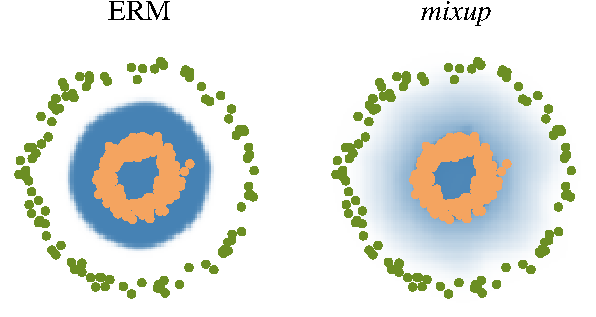
\includegraphics[width=\textwidth]{{images/demo}.pdf}
    \caption{Effect of \mixup{} ($\alpha=1$) on a toy problem. Green: Class 0. Orange: Class 1. Blue shading indicates $p(y=1|x)$.}
    \label{fig:mixup:toy}
\end{subfigure}
\label{fig:mixup}
\vspace{-15pt}
\caption{Illustration of \mixup{}, which converges to ERM as $\alpha \to 0$.}
\end{figure}

\paragraph{What is \mixup{} doing?} The \mixup{} vicinal distribution can be
understood as a form of data augmentation that encourages the model $f$ to
behave linearly in-between training examples. We argue that this linear
behaviour reduces the amount of undesirable oscillations when predicting
outside the training examples. Also, linearity is a good inductive bias from
the perspective of Occam's razor, since it is one of the simplest possible
behaviors. Figure~\ref{fig:mixup:toy} shows that \mixup{} leads to decision
boundaries that transition linearly from class to class, providing a smoother
estimate of uncertainty. Figure~\ref{fig:cifar10_interp} illustrate the average
behaviors of two neural network models trained on the CIFAR-10 dataset using
ERM and \mixup{}.  Both models have the same architecture, are trained with the
same procedure, and are evaluated at the same points in-between randomly
sampled training data.  The model trained with \mixup{} is more stable in terms
of model predictions and gradient norms in-between training samples.

\begin{figure}
	\begin{subfigure}[t]{0.48\textwidth}
		\centering
		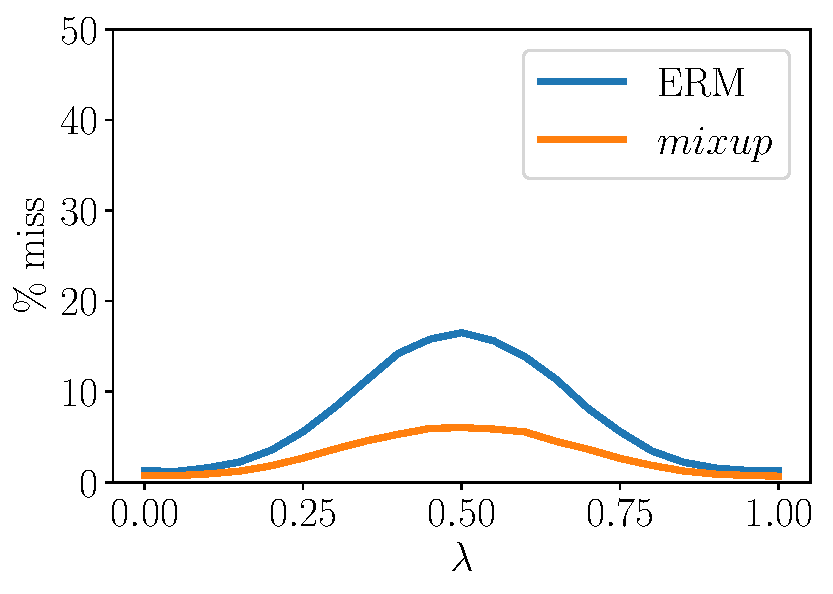
\includegraphics[width=0.75\textwidth]{{images/cifar10_training_interp_miss}.pdf}
        \caption{Prediction errors in-between training data. Evaluated
        at $x = \lambda x_i + (1-\lambda)x_j$, a prediction is counted as a
        ``miss'' if it does not belong to $\{y_i, y_j\}$. The model trained
        with \mixup{} has fewer misses.}
		\label{fig:cifar10_interp:miss}
	\end{subfigure}
	\hfill
	\begin{subfigure}[t]{0.48\textwidth}
		\centering
		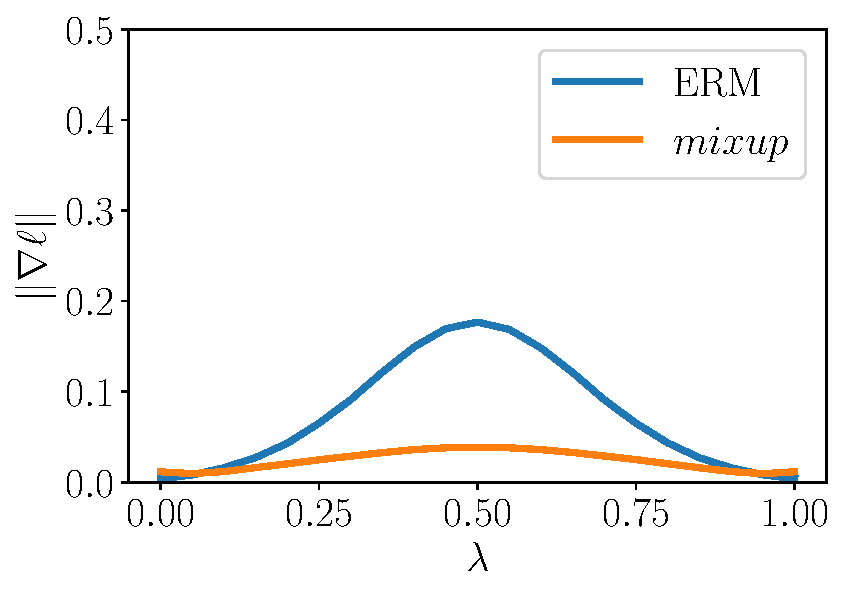
\includegraphics[width=0.75\textwidth]{{images/cifar10_training_interp_norm}.pdf}
        \caption{Norm of the gradients of the model w.r.t. input in-between training data,
        evaluated at $x = \lambda x_i + (1-\lambda)x_j$. The model trained with
        \mixup{} has smaller gradient norms.}
		\label{fig:cifar10_interp:norm}
	\end{subfigure}
	\caption{\mixup{} leads to more robust model behaviors in-between the training data.}
	\label{fig:cifar10_interp}
\end{figure}
